\documentclass{article}
\usepackage[a4paper, left=1.5cm, right=1.5cm, top=1cm, bottom=2cm]{geometry}

\usepackage{boldline}
\usepackage{tikz,tcolorbox}
\usepackage{amsmath}
\usepackage[table,xcdraw]{xcolor}
\usepackage{listings}
\usepackage{array,multirow} % For customizing tables
\usepackage{booktabs} % For better horizontal lines
\usepackage{makecell}
\setlength{\parindent}{0pt}
\usepackage{siunitx}
\usepackage{tkz-tab}
\usepackage{amssymb}
\usepackage{amsmath}
\usepackage{enumitem}

\usepackage{caption}
\usepackage{float}


\newcommand{\exer}[1]{
  \section*{Exercice #1}
  \vspace{-0.5cm}
  \noindent\rule{\textwidth}{0.5pt}%
}

\newcommand{\tit}[1]{
\begin{center}
    \Large{\textbf{{#1}}}
\end{center}
}

\definecolor{commentgray}{HTML}{676160}
\definecolor{messagegreen}{HTML}{17B867}
\definecolor{myblue}{HTML}{10C2C4}

\tcbuselibrary{skins, breakable, theorems}


\newtcolorbox{prettyBox}[2]{
  enhanced,
  colback=white!90!#2,   % Background color based on the second parameter (color)
  colframe=#2!60!black,  % Frame color based on the second parameter (color)
  coltitle=white,        % Title color (white)
  fonttitle=\bfseries\Large,
  title=#1,              % Title from the first parameter
  boxrule=1mm,
  arc=0.5mm,
  drop shadow=#2!35!gray, % Drop shadow color based on the second parameter (color)
}



\lstdefinestyle{cmd}{
 basicstyle=\ttfamily,
 backgroundcolor=\color{lightgray!20},
 frame=single
}

\lstdefinestyle{pythonstyle}{
    language=python,                    % Language set to Python
    basicstyle=\ttfamily\footnotesize,   % Change basic font size
    keywordstyle=\color{blue}\bfseries, % Different keyword style
    stringstyle=\color{red},         % Different string color
    commentstyle=\color{green!60!black}\itshape, % Adjust comment color
    numbers=left,                       % Line numbers on the left
    numberstyle=\tiny\color{gray},      % Smaller number font and color
    stepnumber=1,                       % Number each line
    frame=single,                       % Single frame around code
    tabsize=4,                          % Adjust tab size
    showstringspaces=false,             % Do not show spaces in strings
    captionpos=b,% Position of caption
    breaklines=true,
    inputencoding=utf8
}


\usepackage{tikz}
\usetikzlibrary{arrows.meta, positioning}

\begin{document}

\tit{TD N\(^{\boldsymbol{\circ}}\)\hspace{0.1cm}5}


\begin{prettyBox}{Diagramme de ressources}{myblue}
Le diagramme de ressources permet de représenter l’intensité d’exploitation des ressources pour chaque tâche au cours du temps.  
L’axe des abscisses (x) représente le temps, tandis que l’axe des ordonnées (y) représente les ressources ainsi que leur niveau d’utilisation.\\[0.15cm]
Chaque rectangle correspond à une tâche : sa largeur indique la durée de la tâche, et sa hauteur représente l’intensité d’exploitation de la ressource concernée.\\[0.15cm]
Ce diagramme est utilisé pour détecter les situations de surcharge, c’est-à-dire lorsque l’utilisation d’une ressource dépasse sa capacité maximale.\\[0.15cm]
Pour dessiner le diagram on a besoin du graph PERT pour les date plus tot et les marges total.
\end{prettyBox}

\begin{figure}[H] 
  \centering 
  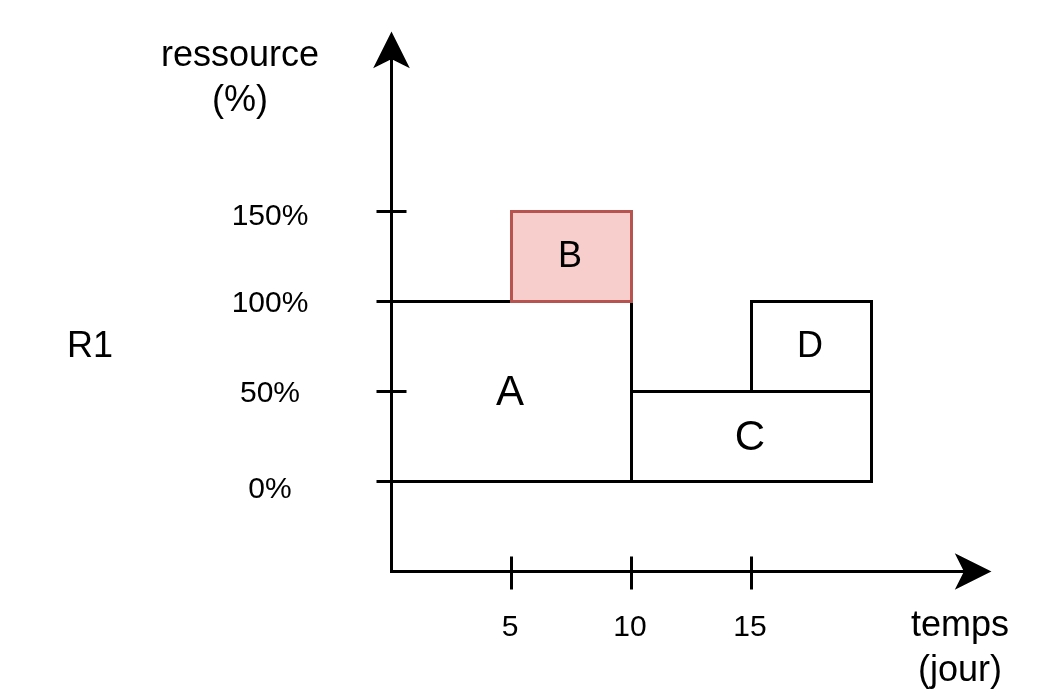
\includegraphics[width=0.55\textwidth]{r1.png} 
\end{figure}

On remarque qu'il ya une surchage de la ressource R1 entre 5-10.

\vspace{0.35cm}


\begin{prettyBox}{Méthodes de traitement des surcharges}{myblue}
Il existe deux principales méthodes de traitement des surcharges de ressources :

\begin{itemize}
    \item \textbf{Lissage} : Le lissage consiste à répartir la charge de travail des ressources en décalant certaines tâches.  
La date de fin du projet est respectée donc les tâches critiques ne sont donc pas décalées et des surcharges peuvent rester si ils affectent la date fin projet.
    \item \textbf{Nivellement} :  
    Le nivellement vise à limiter le nombre de ressources utilisées, ce qui entraîne généralement un allongement de la durée du projet.  
    Cette méthode est appliquée lorsque les ressources disponibles sont limitées.
    
    \begin{itemize}
        \item \textbf{Nivellement par durée} :  
        Les durées des tâches ne sont pas modifiées , seules des décalages sont appliqués afin d’éliminer les surcharges.
        
        \item \textbf{Nivellement par charge} :  
        Le décalage des tâches n’est effectué que si nécessaire. Cette méthode modifie la durée et l’intensité d’exploitation des tâches afin de traiter les surcharges avec
        les formules suivantes :
        \[
        Q = D_{\text{courant}} \times I_{\text{courant}}
        \]
        \[
        I_{\text{nouveau}} = \text{Limite}_{\text{Ressource}} - I_{\text{tâches chevauchantes}}
        \]
        \[
        D_{\text{nouveau}} = \frac{Q}{I_{\text{nouveau}}}
        \]
        \begin{itemize}
            \item $I$ : intensité d’exploitation de la ressource pour une tâche ;
            \item $D$ : durée de la tâche ;
            \item $Q$ : quantité de travail nécessaire pour réaliser la tâche.
        \end{itemize}
    \end{itemize}
\end{itemize}
\end{prettyBox}



\begin{prettyBox}{Règles}{myblue}
\begin{itemize}
    \item On privilégie le décalage ou la modification de la durée des tâches disposant de la plus grande marge totale.
    
    \item On évite de décaler ou de modifier la durée des tâches critiques, car cela affecterait la date de fin du projet.  
    Dans le cas du lissage, ces tâches ne sont jamais décalées , en cas de nivellement elles ne sont modifiées qu’en dernier recours et uniquement si cela est nécessaire.
    
    \item Il est impératif de respecter les liens et les relations de précédence entre les tâches.
\end{itemize}
\end{prettyBox}

\vspace{1.5cm}

\exer{1}

\vspace{0.25cm}

Faite le diagrames des ressource avec ce diagram PERT :

\begin{figure}[H] 
  \centering 
  
\includegraphics[width=0.8\textwidth]{pert1.png} 
\end{figure}


\newpage

\begin{figure}[H] 
  \centering 
  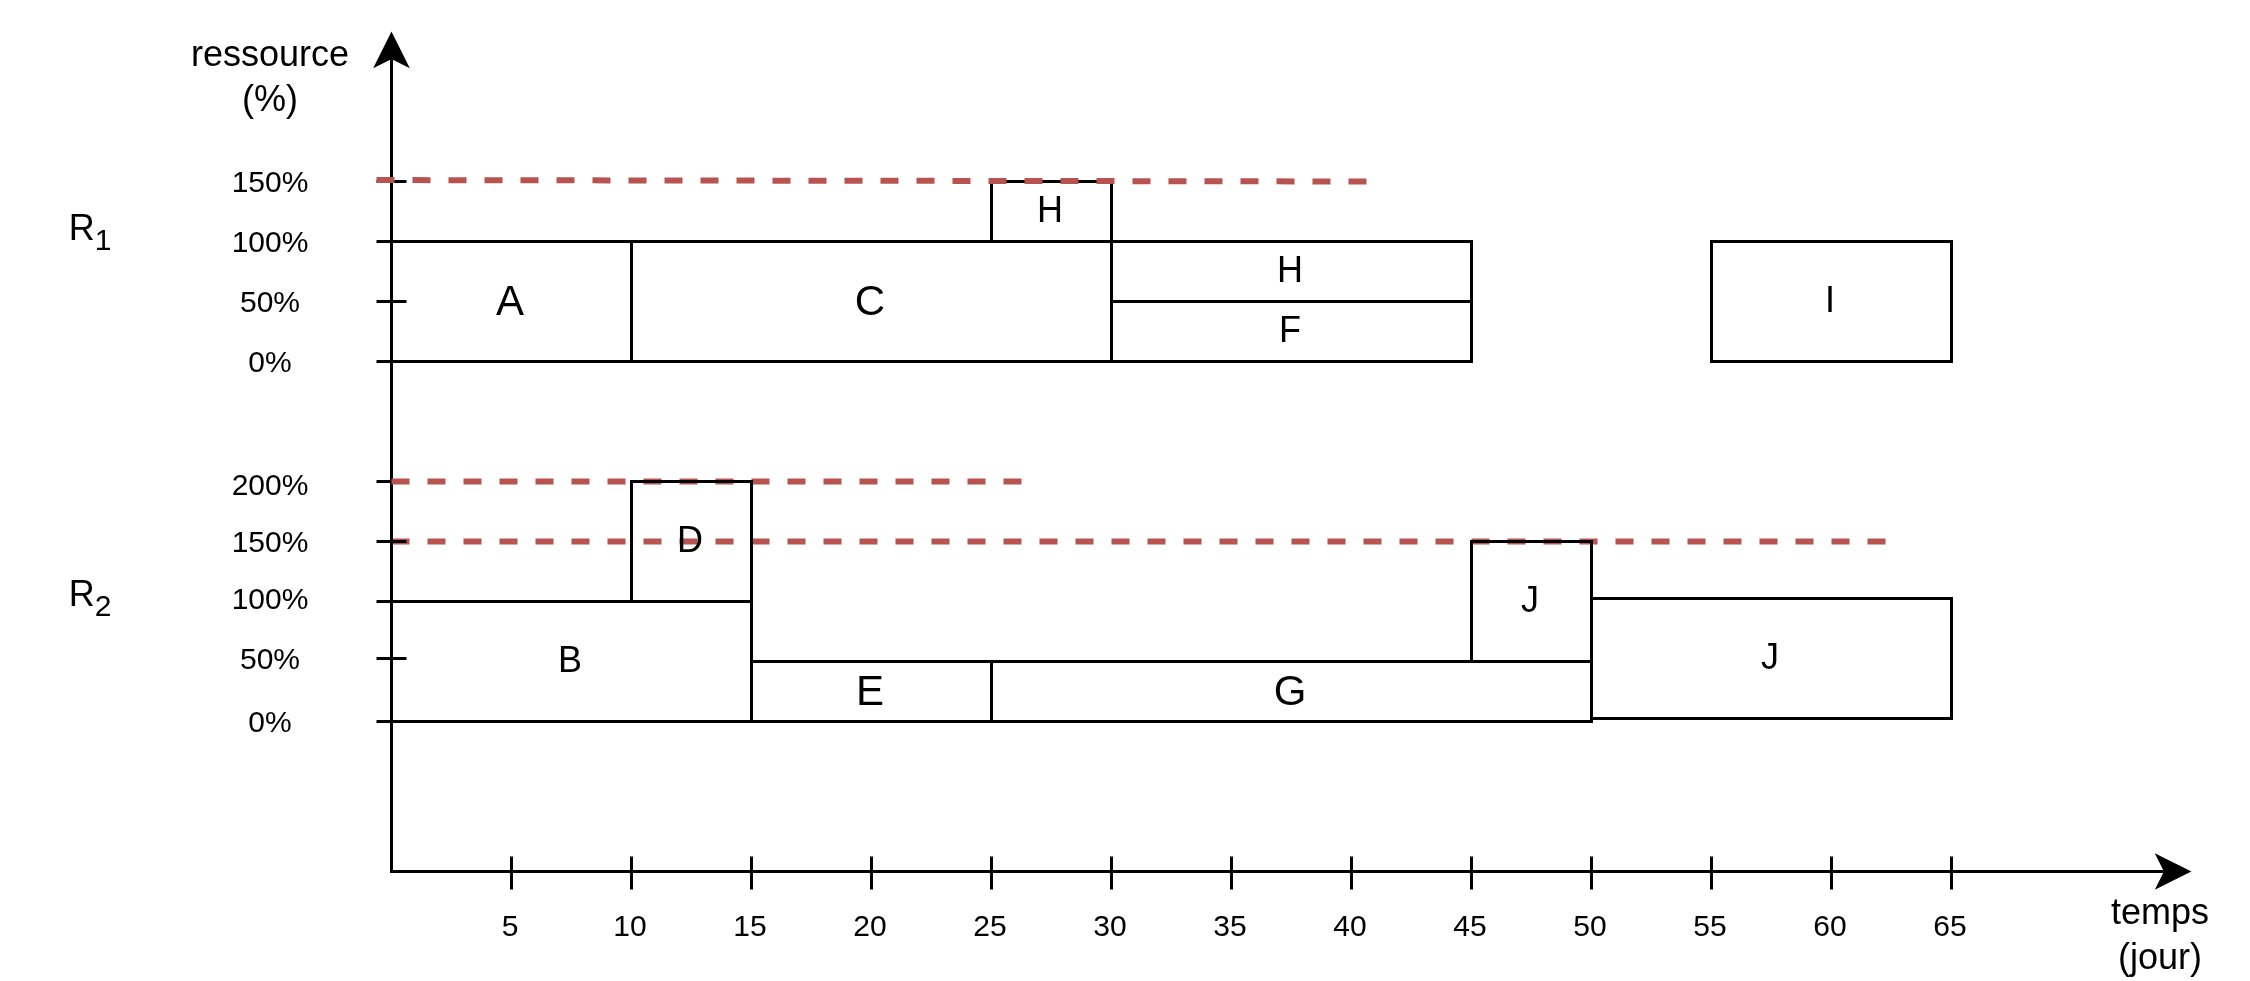
\includegraphics[width=0.8\textwidth]{r2.png} 
\end{figure}

On remarque qu'on a 3 surchage : H , D , J.\\[0.35cm]
\textbf{Nivellement par charge} :  \\[0.15cm]
On va decaler la tache D de 5 Jour n'affecte pas les autre tache car.\\[0.1cm]
On va decaler la tache H de 5 Jour elle va affecter les taches G ,J , I.  
\begin{figure}[H] 
  \centering 
  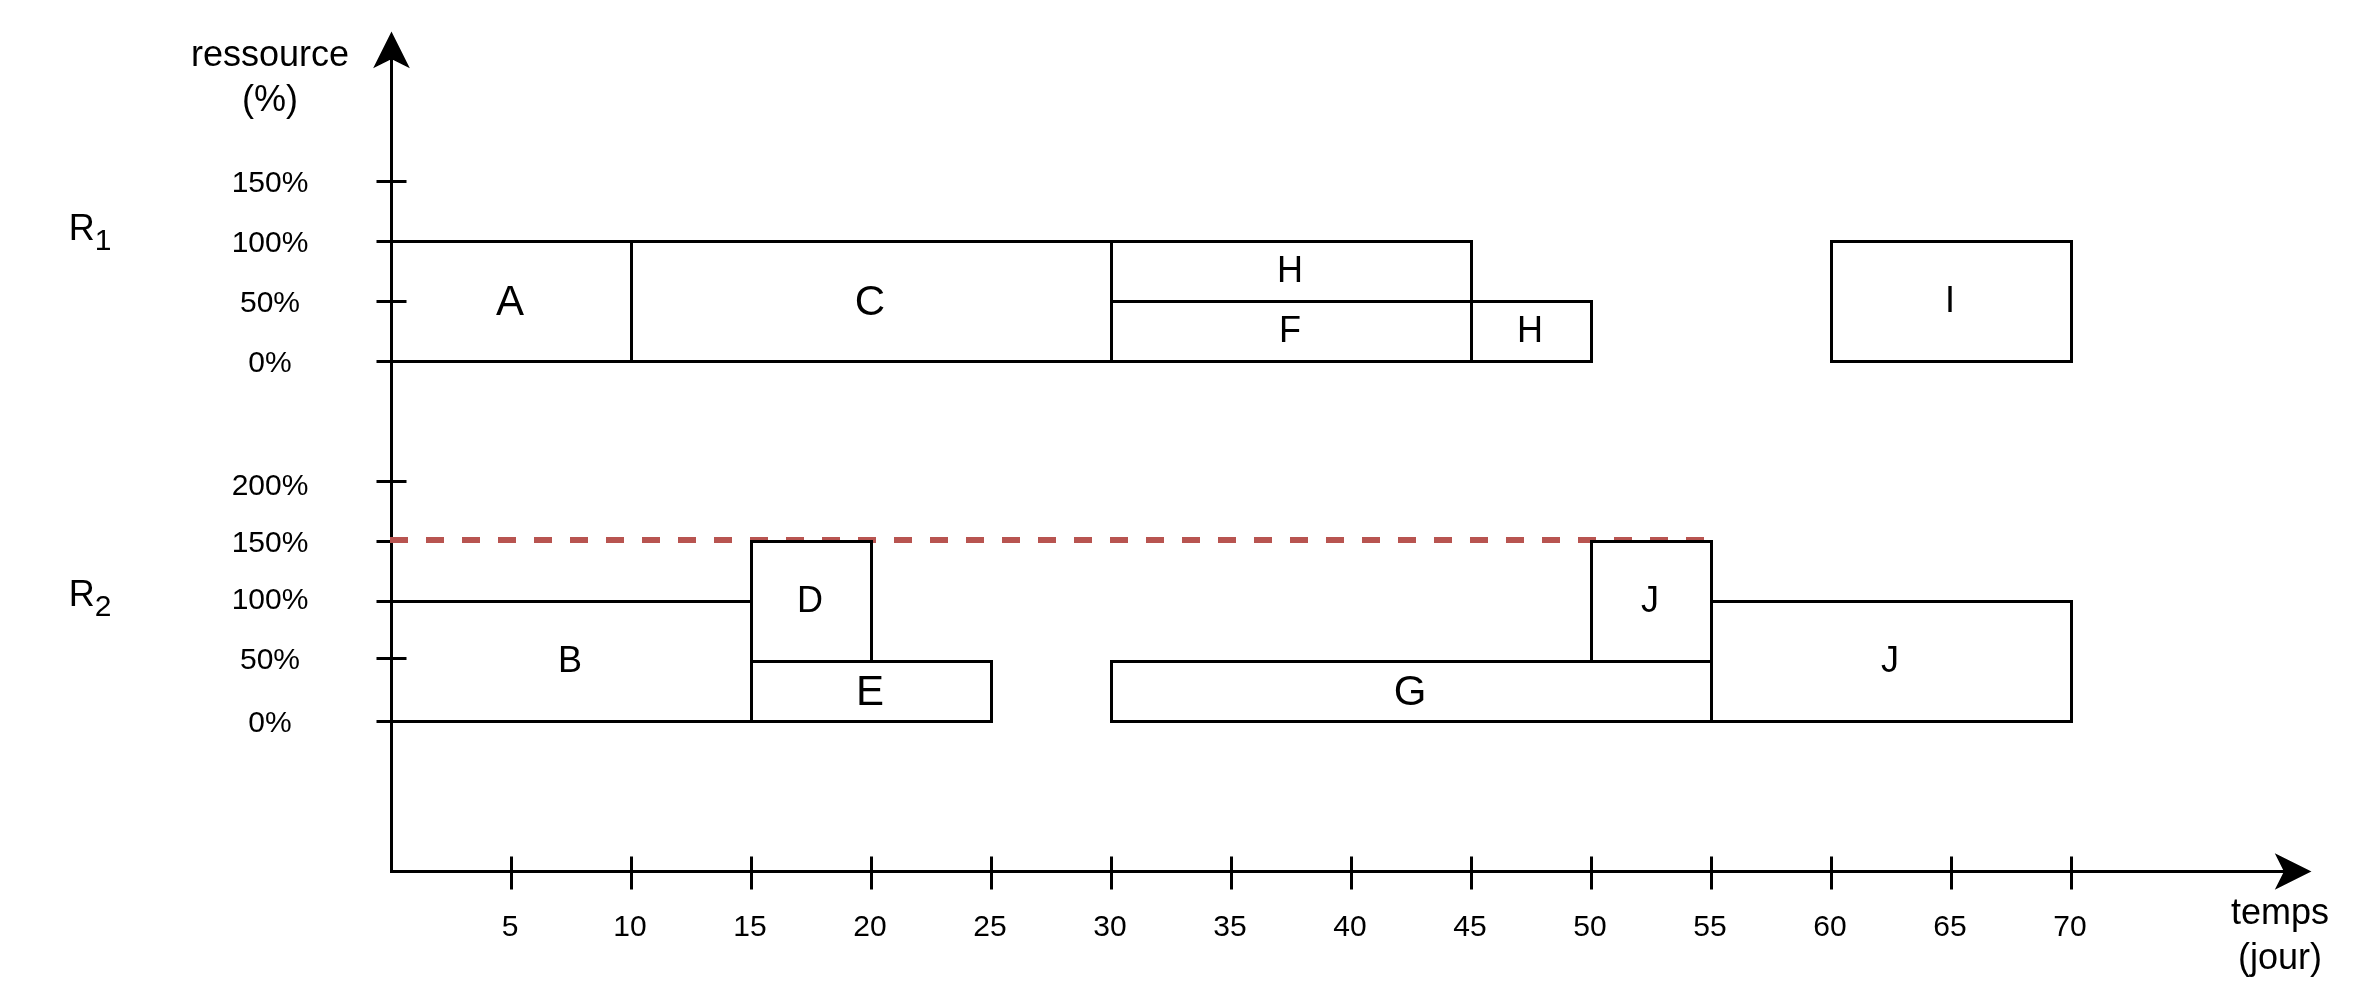
\includegraphics[width=0.8\textwidth]{r3.png} 
\end{figure}

On va utilser la formule pour la tache D on a : $I_{\text{courrant}} = 100\%$ , $D_{\text{courrant}} = 5$jours donc :
\begin{alignat*}{2}
    &Q &&= D_{\text{courrant}} \cdot I_{\text{courrant}} = 5 \cdot 100 = 500\\[0.1cm]
    &I_{\text{nouveau}} &&= \text{Limite}_{\text{R}_{2}} - I_{\text{E}} = 100 - 50 = 50\\[0.1cm]
    &D_{nouveau} &&= \dfrac{Q}{I_{\text{nouveau}}} = \dfrac{500}{50} = 10. 
\end{alignat*}

Et on decale J de 5 jours :


\begin{figure}[H] 
  \centering 
  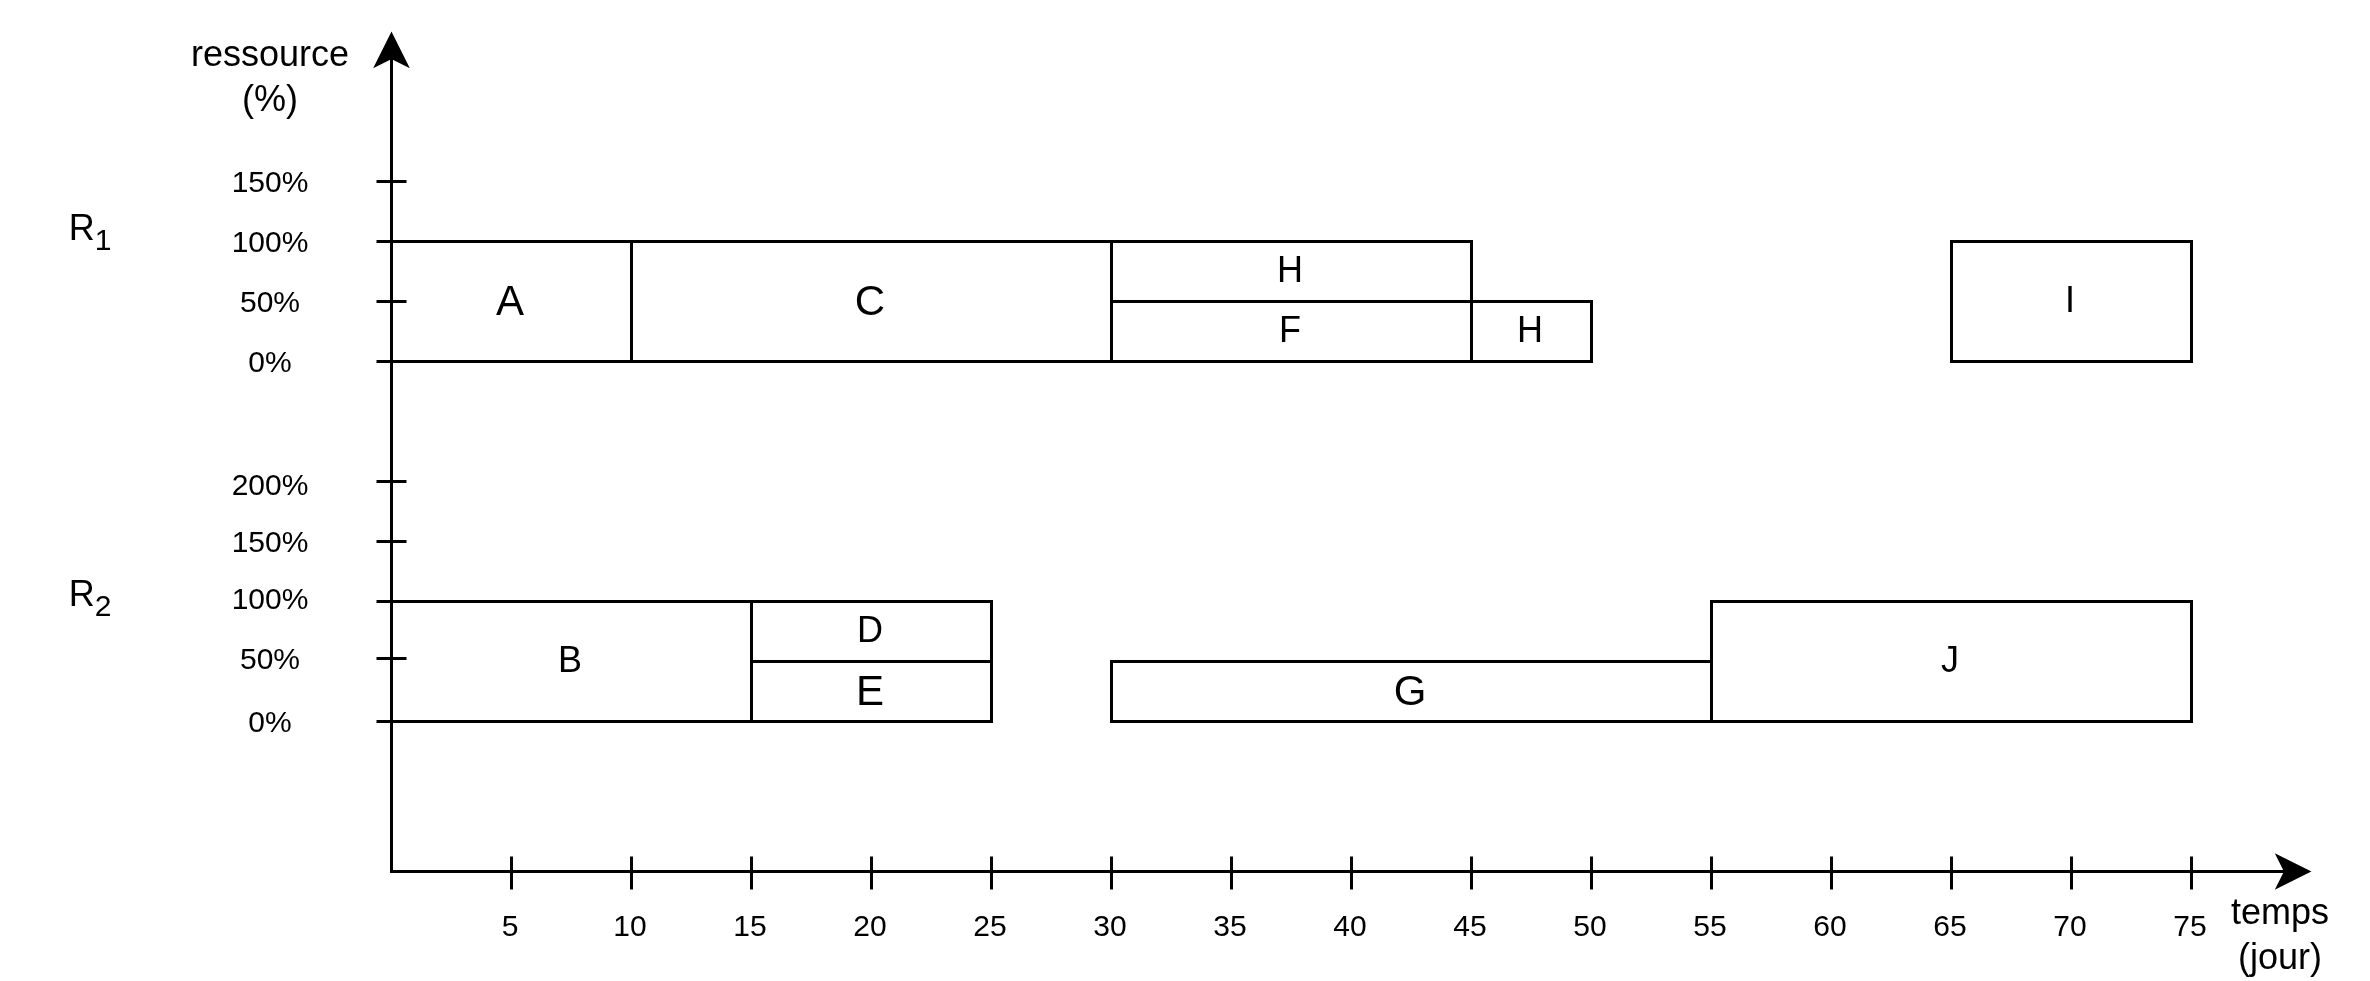
\includegraphics[width=0.8\textwidth]{r4.png} 
\end{figure}

\begin{prettyBox}{Conclusion}{red}
    \begin{itemize}
        \item On a decaler les taches critques H,J de 5 jour (affecte date fin projet).
        \item On a decaler D de 5 jours et on a ajouter 5 jour a ca duree on a consommer tout la marge total 10 (n'affecte pas date fin projet).
        \item Date fin projet est devenue 75.
    \end{itemize}
\end{prettyBox}

\vspace{0.35cm}
\textbf{Nivellement par duree} :  \\[0.15cm]
On va decaler la tache H de 5 Jour elle va affecter les taches G ,J , I.  

\begin{figure}[H] 
  \centering 
  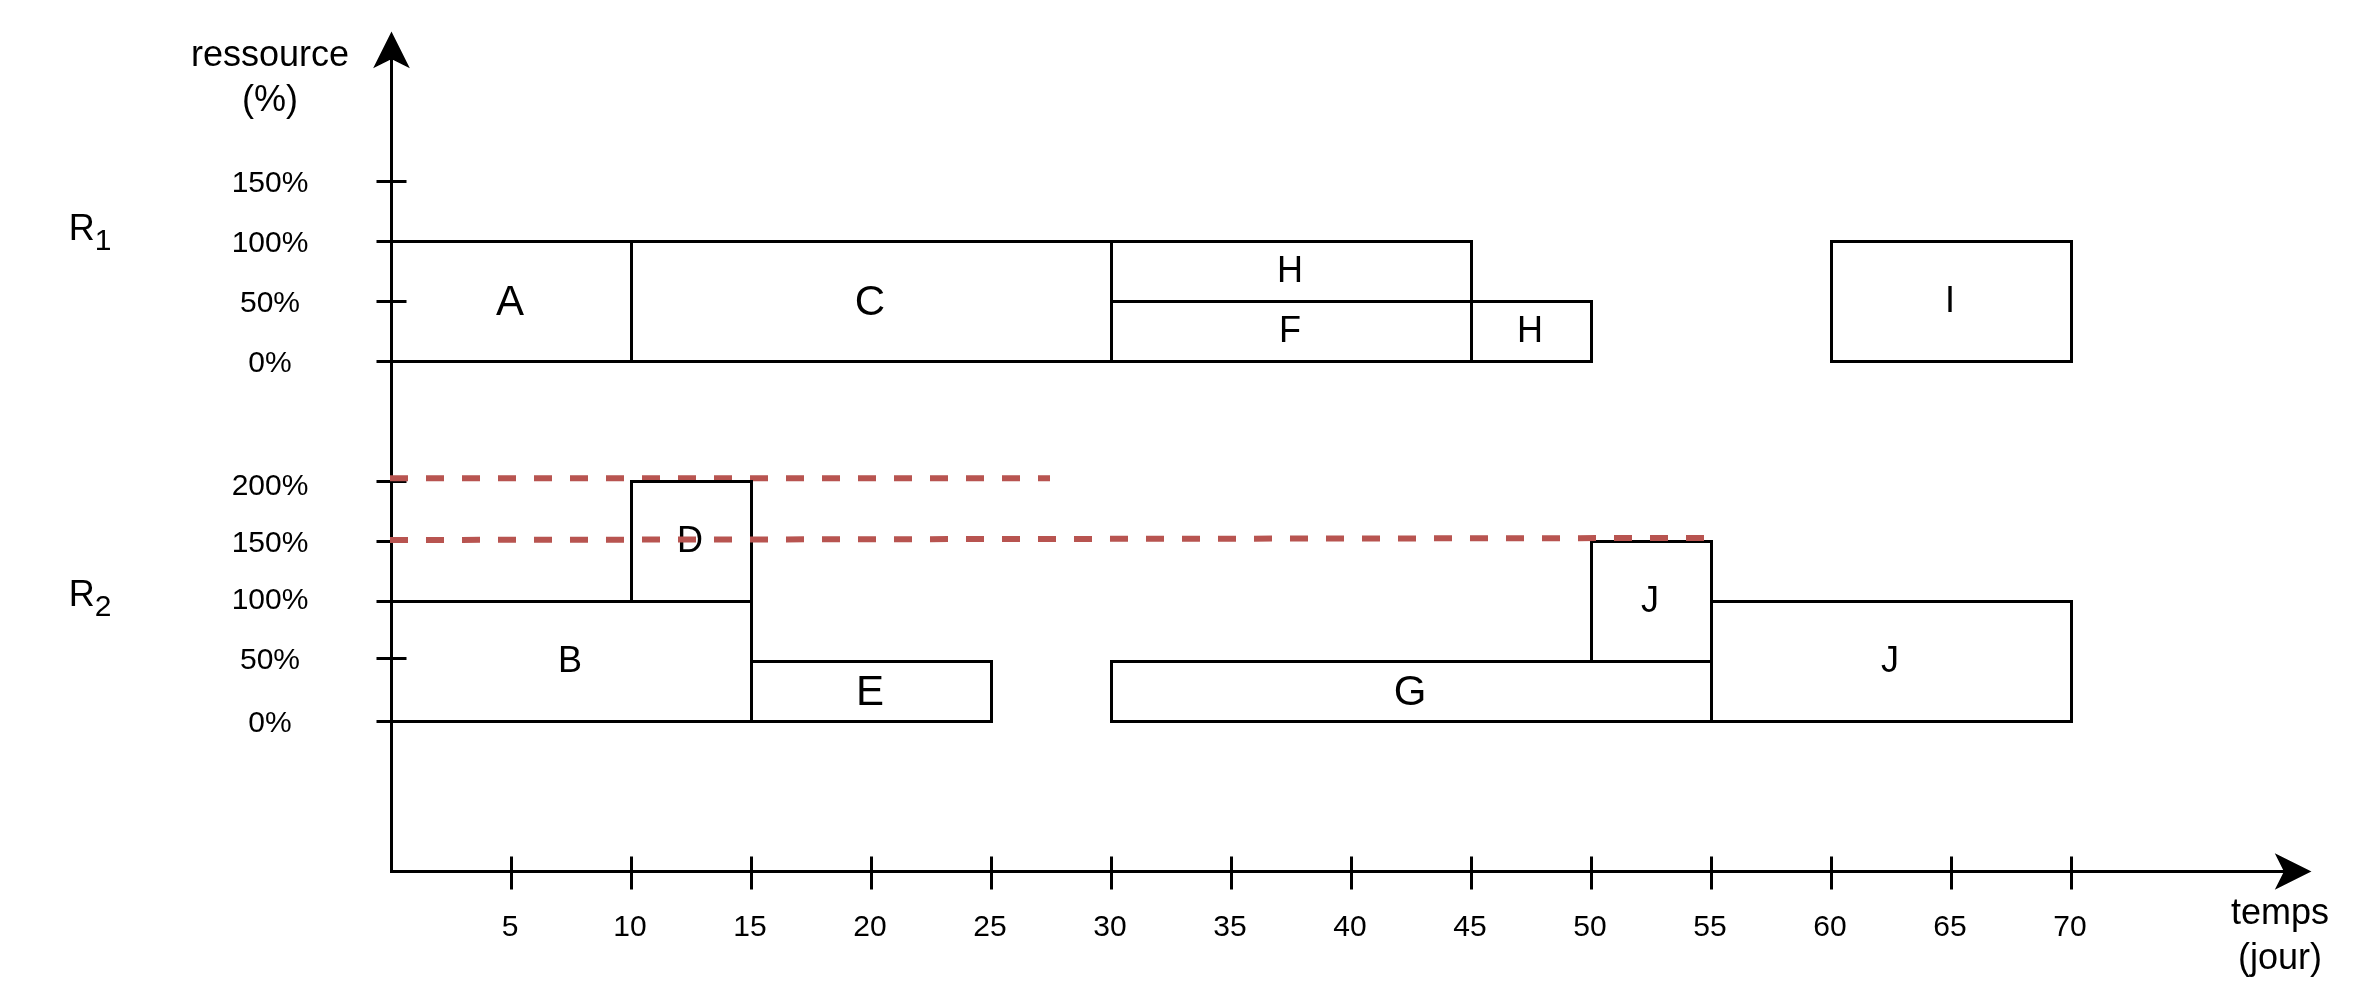
\includegraphics[width=0.8\textwidth]{r5.png} 
\end{figure}

\vspace{0.25cm}


On va decaler la tache D de 15 Jour.\\[0.1cm] 
On va decaler la tache J de 5 Jour elle va affecter la tache I.\\[0.1cm]  

\begin{figure}[H] 
  \centering 
  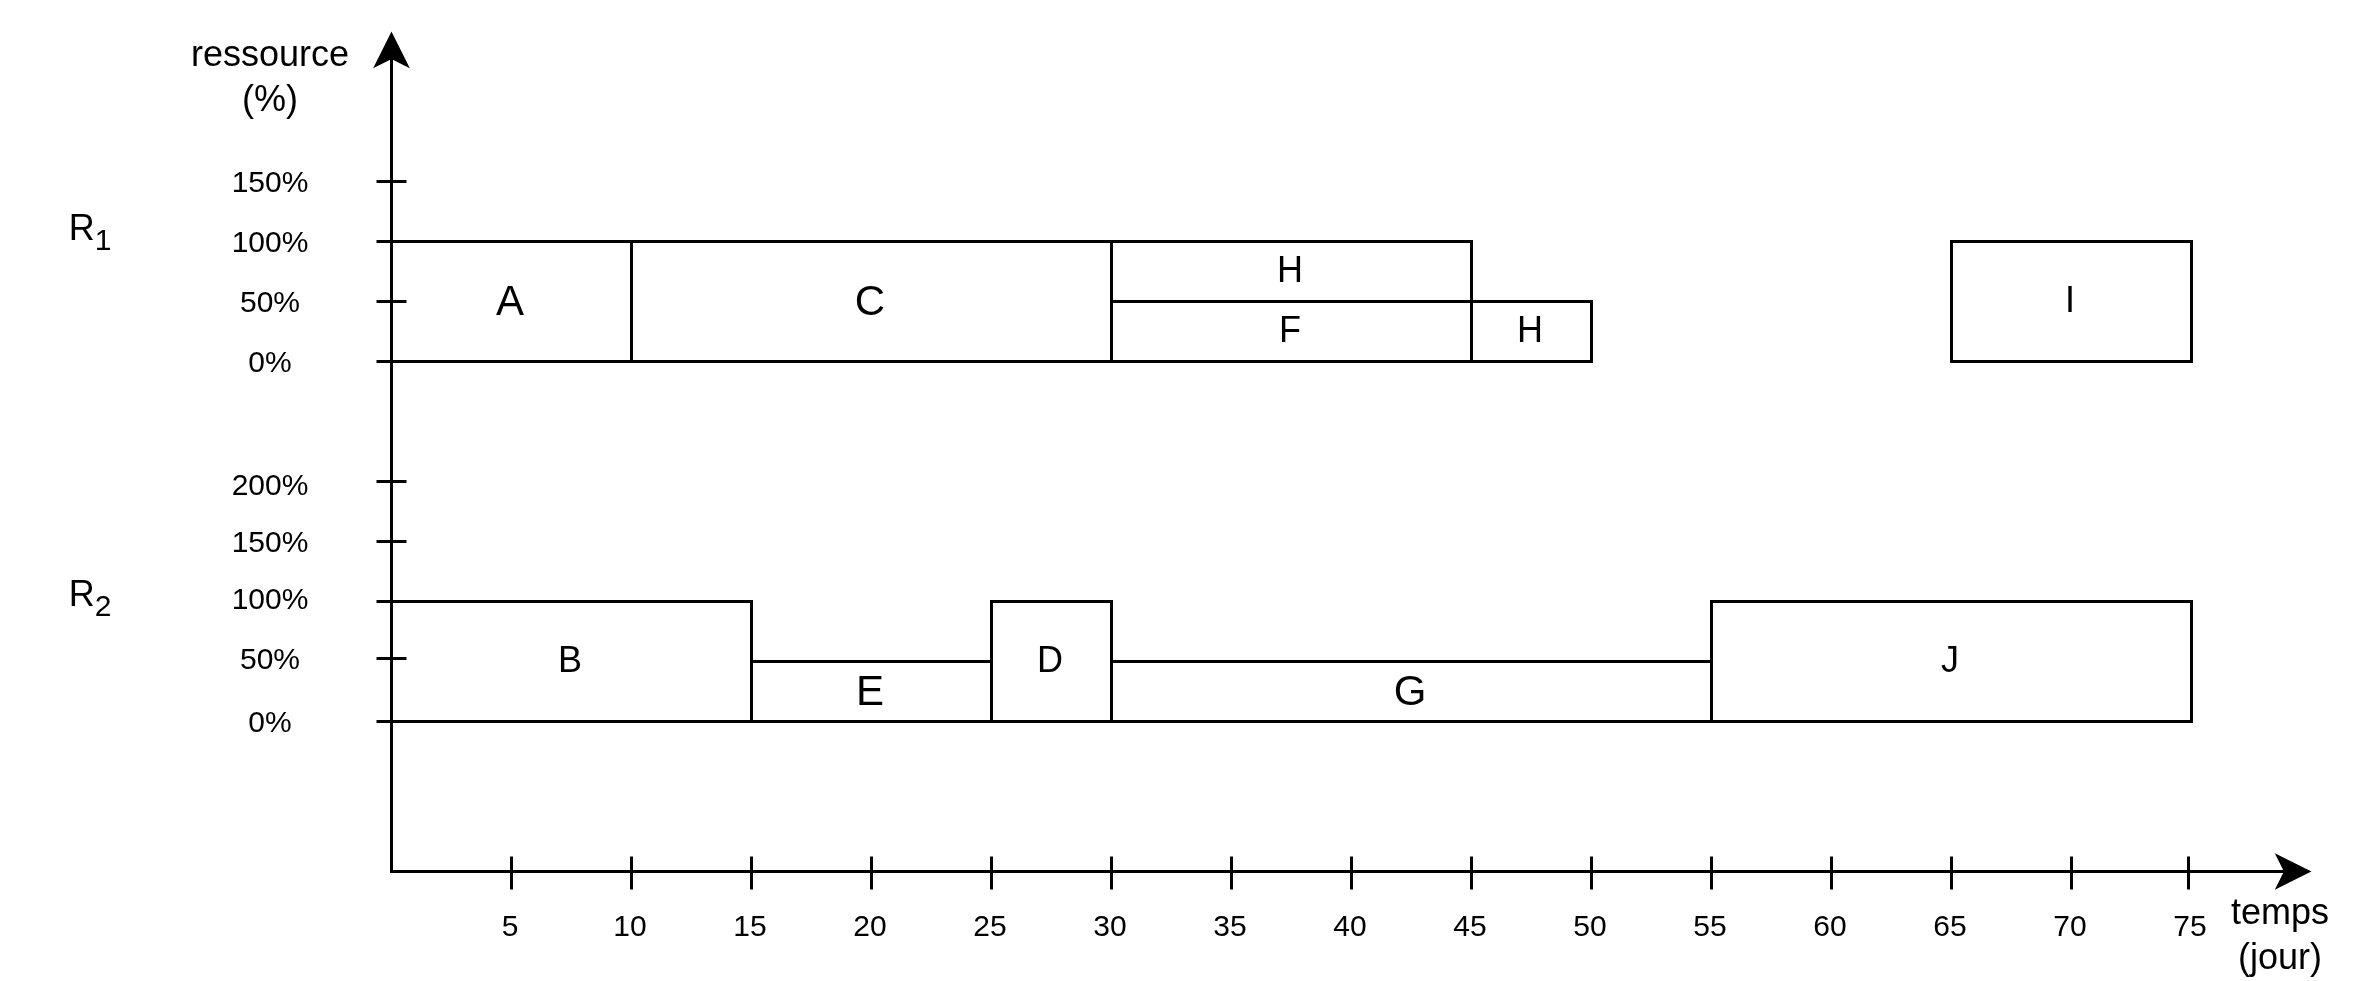
\includegraphics[width=0.8\textwidth]{r6.png} 
\end{figure}


\begin{prettyBox}{Conclusion}{red}
    \begin{itemize}
        \item On a decaler les taches critques H,J de 5 jour (affecte date fin projet).
        \item On a decaler D de 15 jours et on a consommer plus que la marge total 10 (affecte date fin projet).
        \item Date fin projet est devenue 75.
    \end{itemize}
\end{prettyBox}

\newpage

\exer{2}

\vspace{0.25cm}

\begin{figure}[H] 
  \centering 
  
\includegraphics[width=0.3\textwidth]{tab.png} 
\end{figure}


{\LARGE PERT Plus Tot}

\vspace{0.15cm}

\begin{figure}[H] 
  \centering 
  
\includegraphics[width=0.7\textwidth]{pert2.png} 
\end{figure}

\vspace{0.25cm}
{\LARGE PERT Plus Tard}

\vspace{0.15cm}
\begin{figure}[H] 
  \centering 
  
\includegraphics[width=0.7\textwidth]{pert3.png} 
\end{figure}

\newpage
{\LARGE Marges \par}
\begin{itemize}
    \item \textbf{T1} : MT = 0-0 = 3-3 = 0 $\Rightarrow$ ML = 0.
    \item \textbf{T3} : MT = 3-3 = 7-7 = 0 $\Rightarrow$ ML = 0.
    \item \textbf{T4} : MT = 7-7 = 8-8 = 0 $\Rightarrow$ ML = 0.
    \item \textbf{T6} : MT = 8-8 = 11-11 = 0 $\Rightarrow$ ML = 0.
    \item \textbf{T8} : MT = 11-11 = 13-13 = 0 $\Rightarrow$ ML = 0.
    \item \textbf{T10} : MT = 13-13 = 19-19 = 0 $\Rightarrow$ ML = 0.
    \item \textbf{T12} : MT = 19-19 = 22-22 = 0 $\Rightarrow$ ML = 0.
    \item \textbf{T2}: MT= 5-0 = 7-2 = 5  , ML = min(c-e) - Date Debut Plus Tot de T2 = min(2-2,5-2)-0 = 0.
    \item \textbf{T5}: MT= 7-5 = 13-11 = 2  , ML = min(c-e) - Date Debut Plus Tot de T5 = min(13-6)- 5 = 2.
    \item \textbf{T7}: MT= 9-2 = 11-4 = 7  , ML = min(c-e) - Date Debut Plus Tot de T7 = min(11-2)-2 = 7.
    \item \textbf{T9}: MT= 2-0 = 7-5 = 2  , ML = min(c-e) - Date Debut Plus Tot de T9 = min(5-5,5-5)-0 = 0.
    \item \textbf{T11}: MT= 18-5 = 19-6 = 13  , ML = min(c-e) - Date Debut Plus Tot de T11 = min(19-1)-5 = 13.
\end{itemize}

\vspace{0.15cm}

\begin{figure}[H] 
  \centering 
  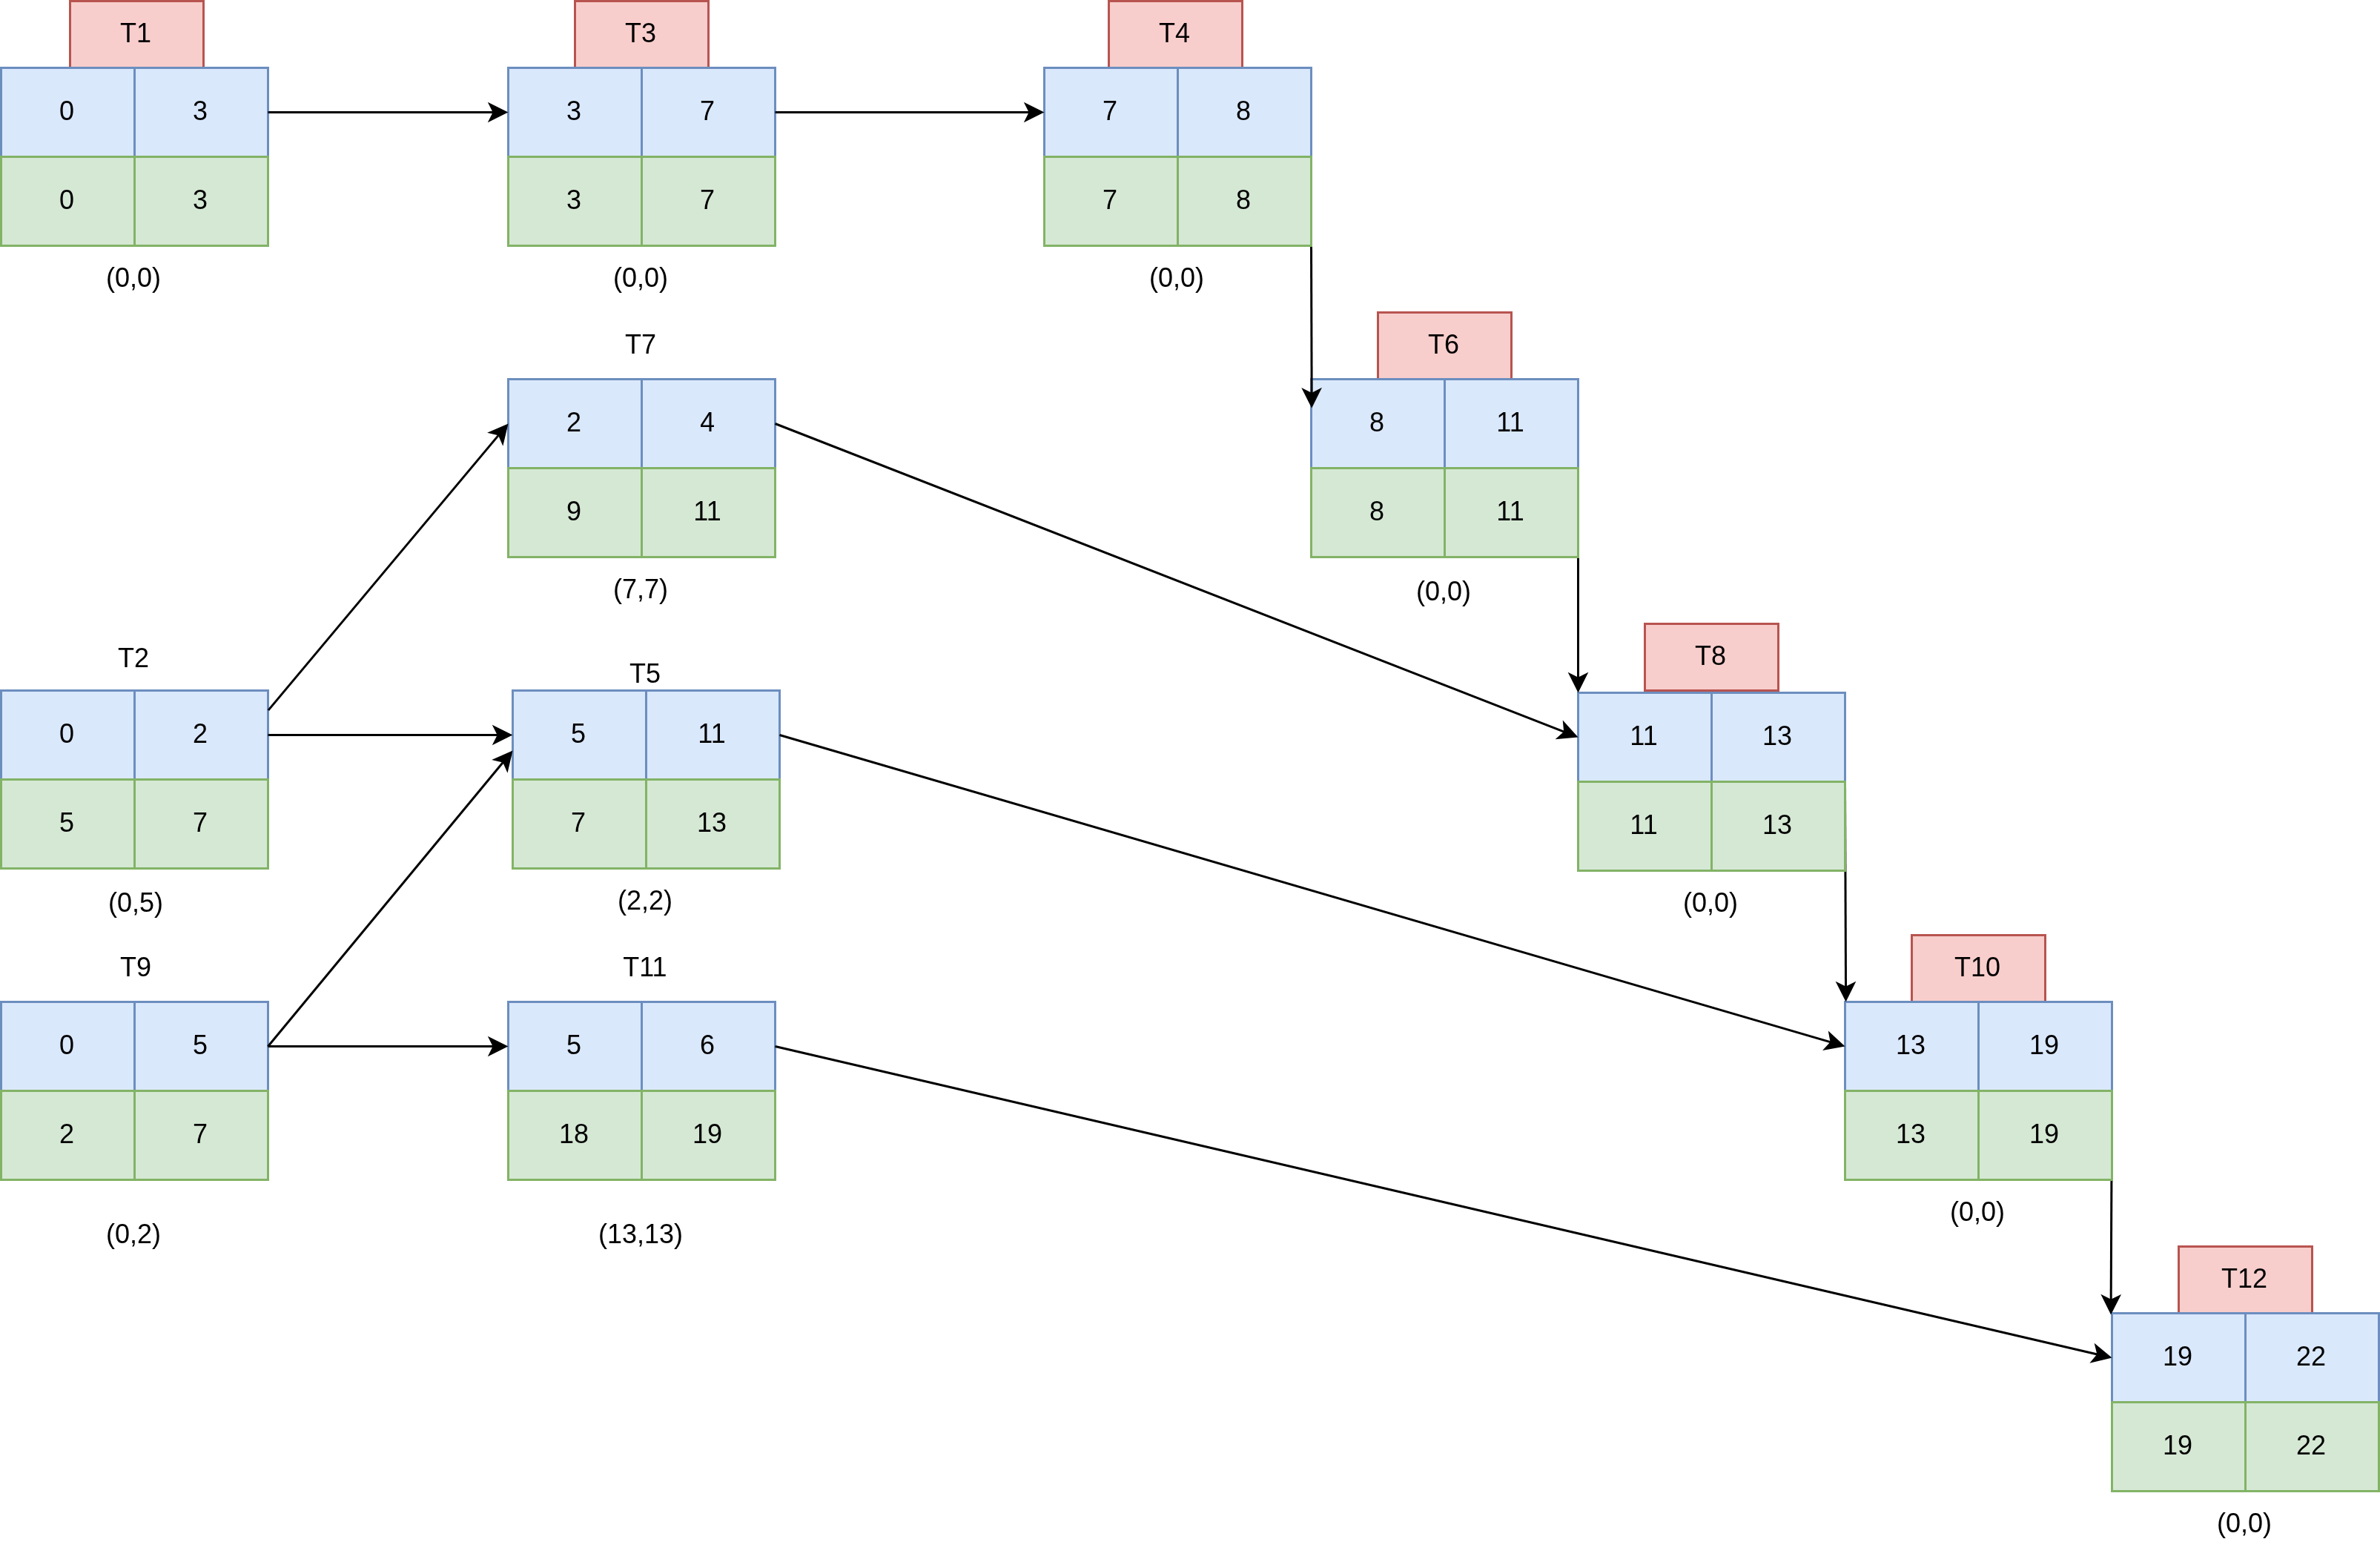
\includegraphics[width=0.8\textwidth]{pert4.png} 
\end{figure}

\vspace{0.15cm}

Taches Critique : T1,T3,T4,T6,T8,T10,T12\\
Chemin Critique : T1 T3 T4 T6 T8 T10 T12\\
Duree du projet : 22jours

\newpage

\begin{figure}[H] 
  \centering 
  
\includegraphics[width=0.6\textwidth]{gant.png} 
\end{figure}

\newpage

\textbf{Nombre de ressource optimal} :\\[0.15cm]
Pour eviter la surchage on va prendre le nombre de ressource = nombre taches en paralleles :\\[0.1cm]
On T1 , T2 , T9 en parallele donc on aura besoin de 3 ressources :

\begin{figure}[H] 
  \centering 
  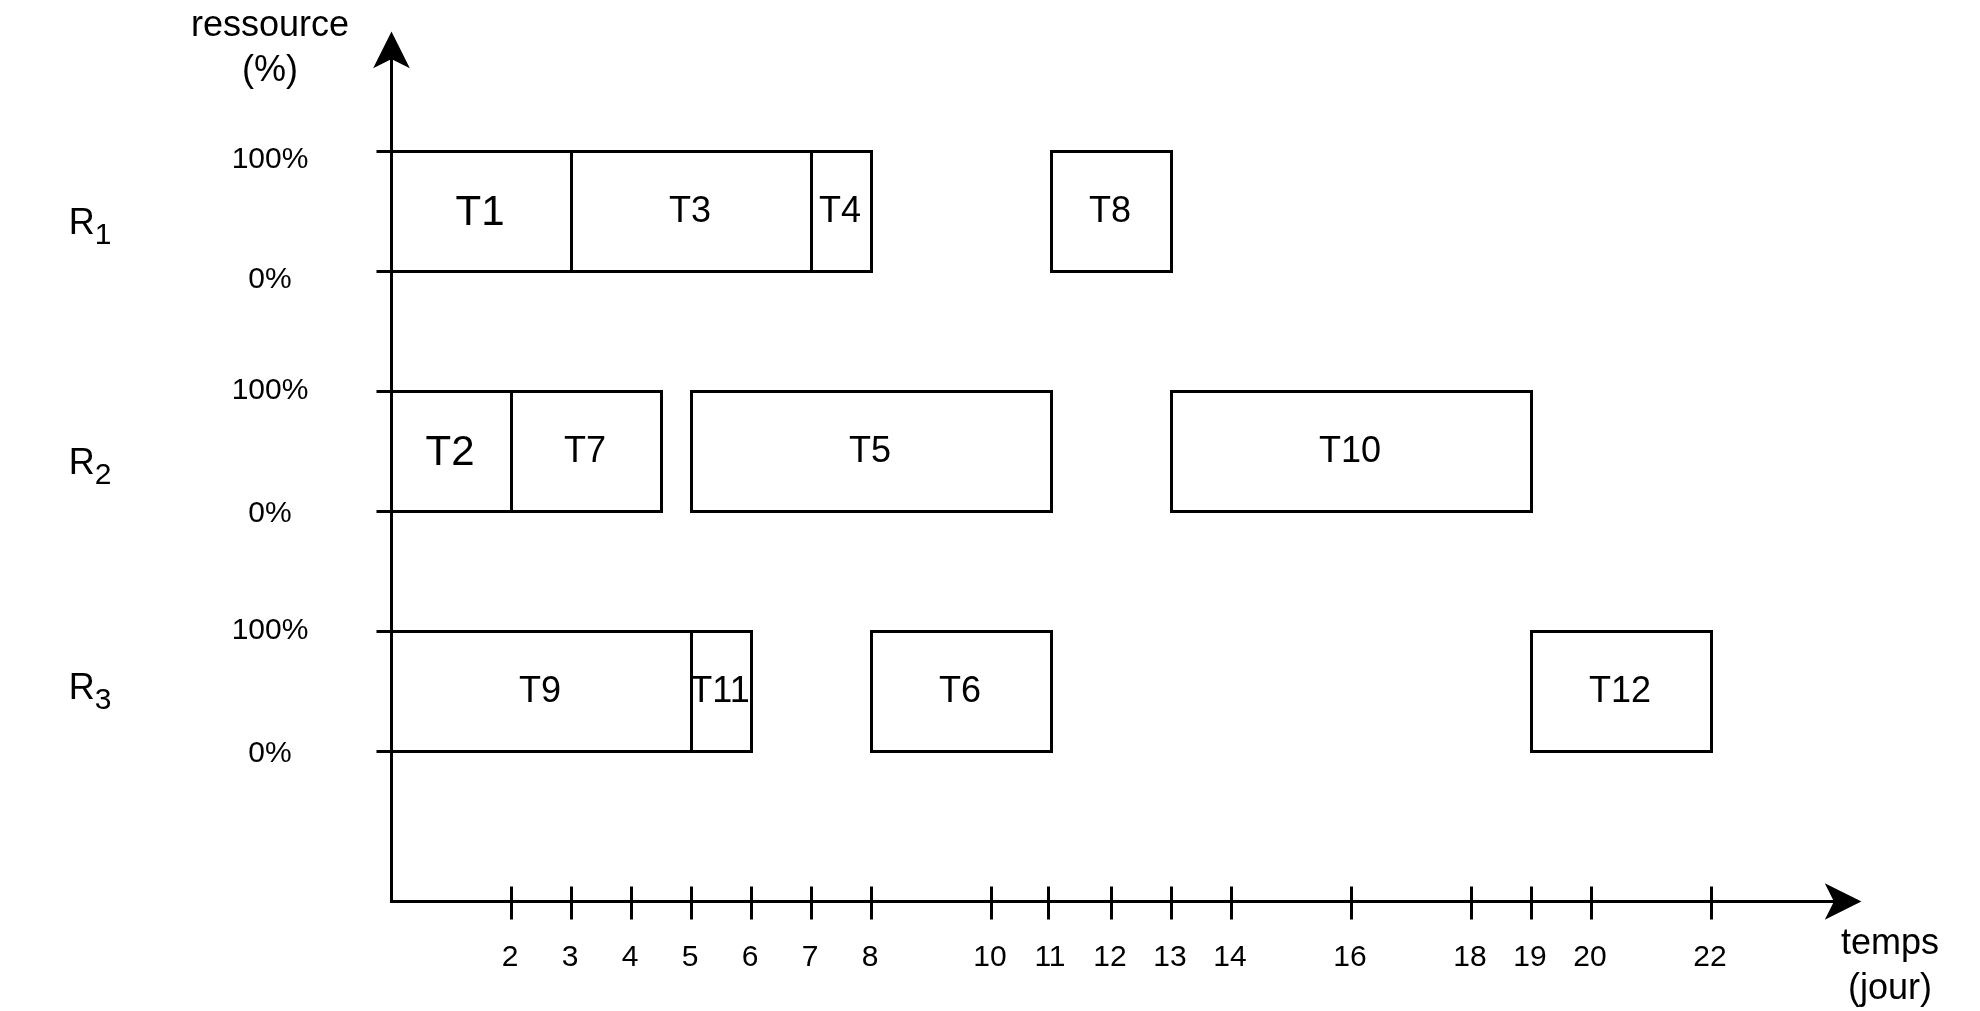
\includegraphics[width=0.8\textwidth]{r.png} 
\end{figure}



\end{document}

